\begin{frame}{Robot Model}
Assume that the robot could not observe its real state directly.  
It make its decisions by maintaining an \emph{I-state} $\eta_k$.
\begin{itemize}
\item State space: $X = \mathbb{R}^2$,  $X_{obt} \cup X_{free} \subseteq X$
\item Action space: $U = \mathbb{R}^2$, apply a bounded noise $\theta_k$ to the
  action $u_k \in U$
\item Set valued state transition function: $F(x, u)$
  \begin{equation}
    \label{eq:state-trans}
    F(x_k, u_k) = \left\{
      x_k + u_k + \theta_k
      \mid
      \theta_k \in \Theta(u_k)
    \right\} \cap X_{free}
  \end{equation}
  \begin{columns}
    \begin{column}{0.4\textwidth}
      \begin{figure}
        \centering
        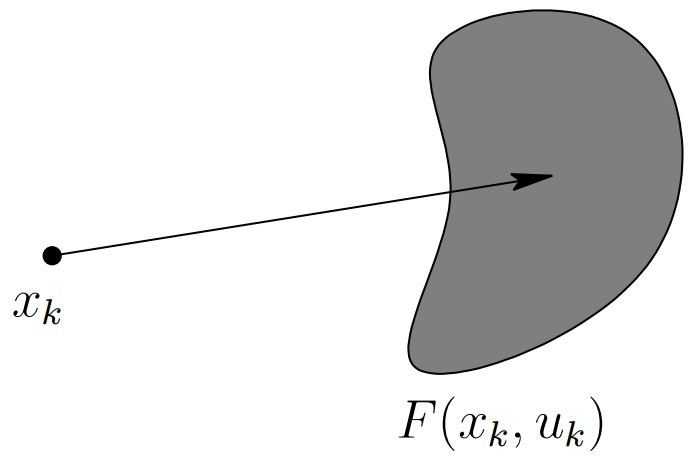
\includegraphics[scale=0.2]{figs/istate.jpg}
        \caption{\scriptsize{The transition of robot's state $x_k$ with
            uncertainty [\emph{Planning Algorithms}, S. LaValle, 2006].}}
      \end{figure}
    \end{column}
    \begin{column}{0.5\textwidth}
      \begin{figure}
        \centering
        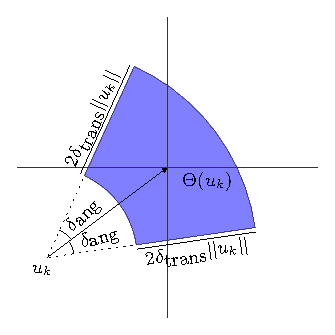
\includegraphics[scale=0.55]{figs/noisemodel}
        \caption{\scriptsize{The noise model $\Theta(u_k)$ involves bounded
            angular error $\delta_{ang}$ and bounded translational error
            $\delta_{trans}||u||$.}}
        \label{fig:noiseModel}
      \end{figure}
    \end{column}
  \end{columns}
\end{itemize}
\end{frame}
